%!TEX root = ../main.tex
\documentclass{beamer} % Gliederung im Kopf, sections und subsections
\renewcommand{\baselinestretch}{1.5}\normalsize
\usetheme{default}
\setbeamertemplate{navigation symbols}{}

\usepackage{tabu}
\usepackage{etex}
%\usepackage{beamerthemesplit}
%\useoutertheme[subsection=false]{smoothbars}
%\usepackage[final]{pdfpages}
\usepackage{bibentry}
\usepackage{bm}
\usepackage{bigints}
\usepackage{graphicx}
\usepackage{relsize}
\usepackage[round,longnamesfirst]{natbib}
\usepackage{bm}																									%matrix symbol
\usepackage{bbm}
\usepackage{verbatim}
\usepackage{setspace}																					%Fußnoten (allgm.
\usepackage{hyperref}
\usepackage{bibentry}
\nobibliography*

\hypersetup{colorlinks=true,urlcolor=blue}														%Zeilenabstände)
\usepackage{threeparttable}
\usepackage{subfig}
\usepackage{epstopdf}
\usepackage{lscape}																							%Querformat
\usepackage[latin1]{inputenc}																		%Umlaute
\usepackage{graphicx}
%\graphicspath{{../shared-files/}}

\usepackage{tikz}
\tikzset{
  treenode/.style = {shape=rectangle, rounded corners,
                     draw, align=center,
                     top color=white, bottom color=blue!20},
  root/.style     = {treenode, font=\Large, bottom color=red!30},
  env/.style      = {treenode, font=\ttfamily\normalsize},
  dummy/.style    = {circle,draw}
}

\usepackage{tikz}
\usetikzlibrary{trees,shapes,arrows,decorations.pathmorphing,backgrounds,positioning,fit,petri}
\renewcommand*{\familydefault}{\sfdefault}

\tikzset{forestyle/.style = {rectangle, thick, minimum width = 5cm, minimum height = 0.5cm, text width = 4.5cm, outer sep = 1mm},
	pre/.style={<-, shorten <=1pt, >=stealth, ultra thick},
	extend/.style={<-,dashed, shorten <=1pt, >=stealth, ultra thick}}
\captionsetup[subfigure]{labelformat=empty}


\mode<presentation>

\begin{document}

\begin{frame}[noframenumbering]\begin{center}

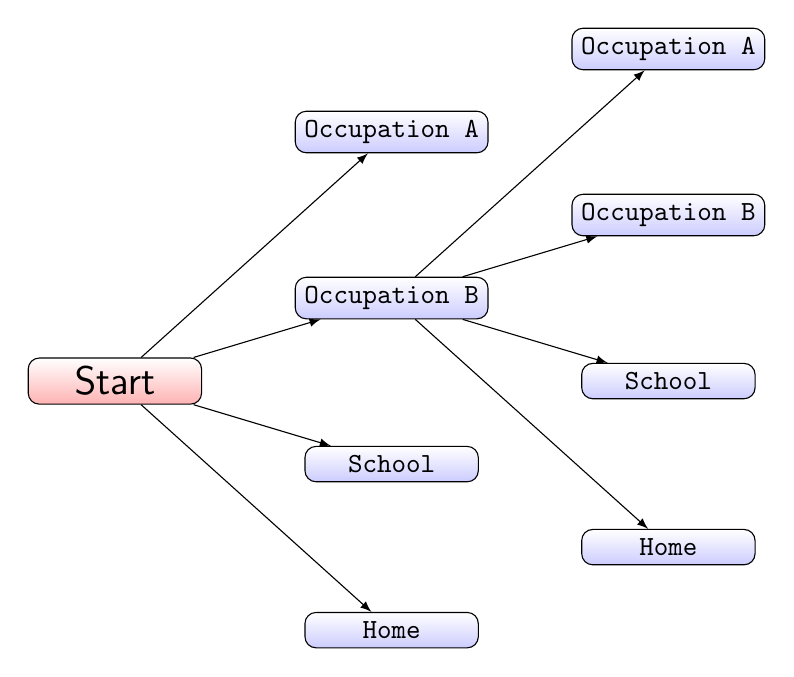
\begin{tikzpicture}
  [
    grow                    = right,
    sibling distance        = 6em,
    level distance          = 10em,
    edge from parent/.style = {draw, -latex},
    every node/.style       = {font=\footnotesize, minimum width={width("Magnetometer")+2pt}},
    sloped
  ]
  \node [root] {Start}
    child { node [env] {Home}}
    child { node [env] {School}}
    child { node [env] {Occupation B}
            child { node [env] {Home}}
            child { node [env] {School}}
            child { node [env] {Occupation B}}
            child { node [env] {Occupation A}}
           }
    child { node [env] {Occupation A}};
\end{tikzpicture}


\end{center}\end{frame}


\end{document}
